% CVPR 2026 Paper Template; see https://github.com/cvpr-org/author-kit

\documentclass[10pt,twocolumn,letterpaper]{article}

%%%%%%%%% PAPER TYPE  - PLEASE UPDATE FOR FINAL VERSION
%\usepackage{cvpr}              % To produce the CAMERA-READY version
% \usepackage[review]{cvpr}      % To produce the REVIEW version
\usepackage[pagenumbers]{cvpr} % To force page numbers, e.g. for an arXiv version

% Import additional packages in the preamble file, before hyperref
\input{preamble}

% It is strongly recommended to use hyperref, especially for the review version.
% hyperref with option pagebackref eases the reviewers' job.
% Please disable hyperref *only* if you encounter grave issues, 
% e.g. with the file validation for the camera-ready version.
%
% If you comment hyperref and then uncomment it, you should delete *.aux before re-running LaTeX.
% (Or just hit 'q' on the first LaTeX run, let it finish, and you should be clear).
\definecolor{cvprblue}{rgb}{0.21,0.49,0.74}
\usepackage[pagebackref,breaklinks,colorlinks,allcolors=cvprblue]{hyperref}

%%%%%%%%% PAPER ID  - PLEASE UPDATE
\def\paperID{232} % *** Enter the Paper ID here
\def\confName{CVPR}
\def\confYear{2026}

%%%%%%%%% TITLE - PLEASE UPDATE
\title{SUPPLEMENTARY MATERIALS for SHOW3D}

%%%%%%%%% AUTHORS - PLEASE UPDATE
\author{%
\hspace*{-8pt}%
\begin{tabular}[t]{c}
Patrick Rim$^{1,2}$\thanks{}\quad\,
Kevin Harris$^{1}$\quad\,
Braden Copple$^{1}$\quad\,
Shangchen Han$^{1}$\quad\,
Xu Xie$^{1}$\quad\,
Ivan Shugurov$^{1}$\\
Sizhe An$^{1}$\quad\,
He Wen$^{1}$\quad\,
Alex Wong$^{2}$\quad\,
Tomas Hodan$^{1}$\quad\,
Kun He$^{1}$\\[0.2cm]
$^{1}$Meta Reality Labs\qquad
$^{2}$Yale University
\end{tabular}
}

\begin{document}

\twocolumn[{%
  \renewcommand\twocolumn[1][]{#1}%
\maketitle
  \vspace{-8pt}
  \begin{center}
    \captionsetup{type=figure}
    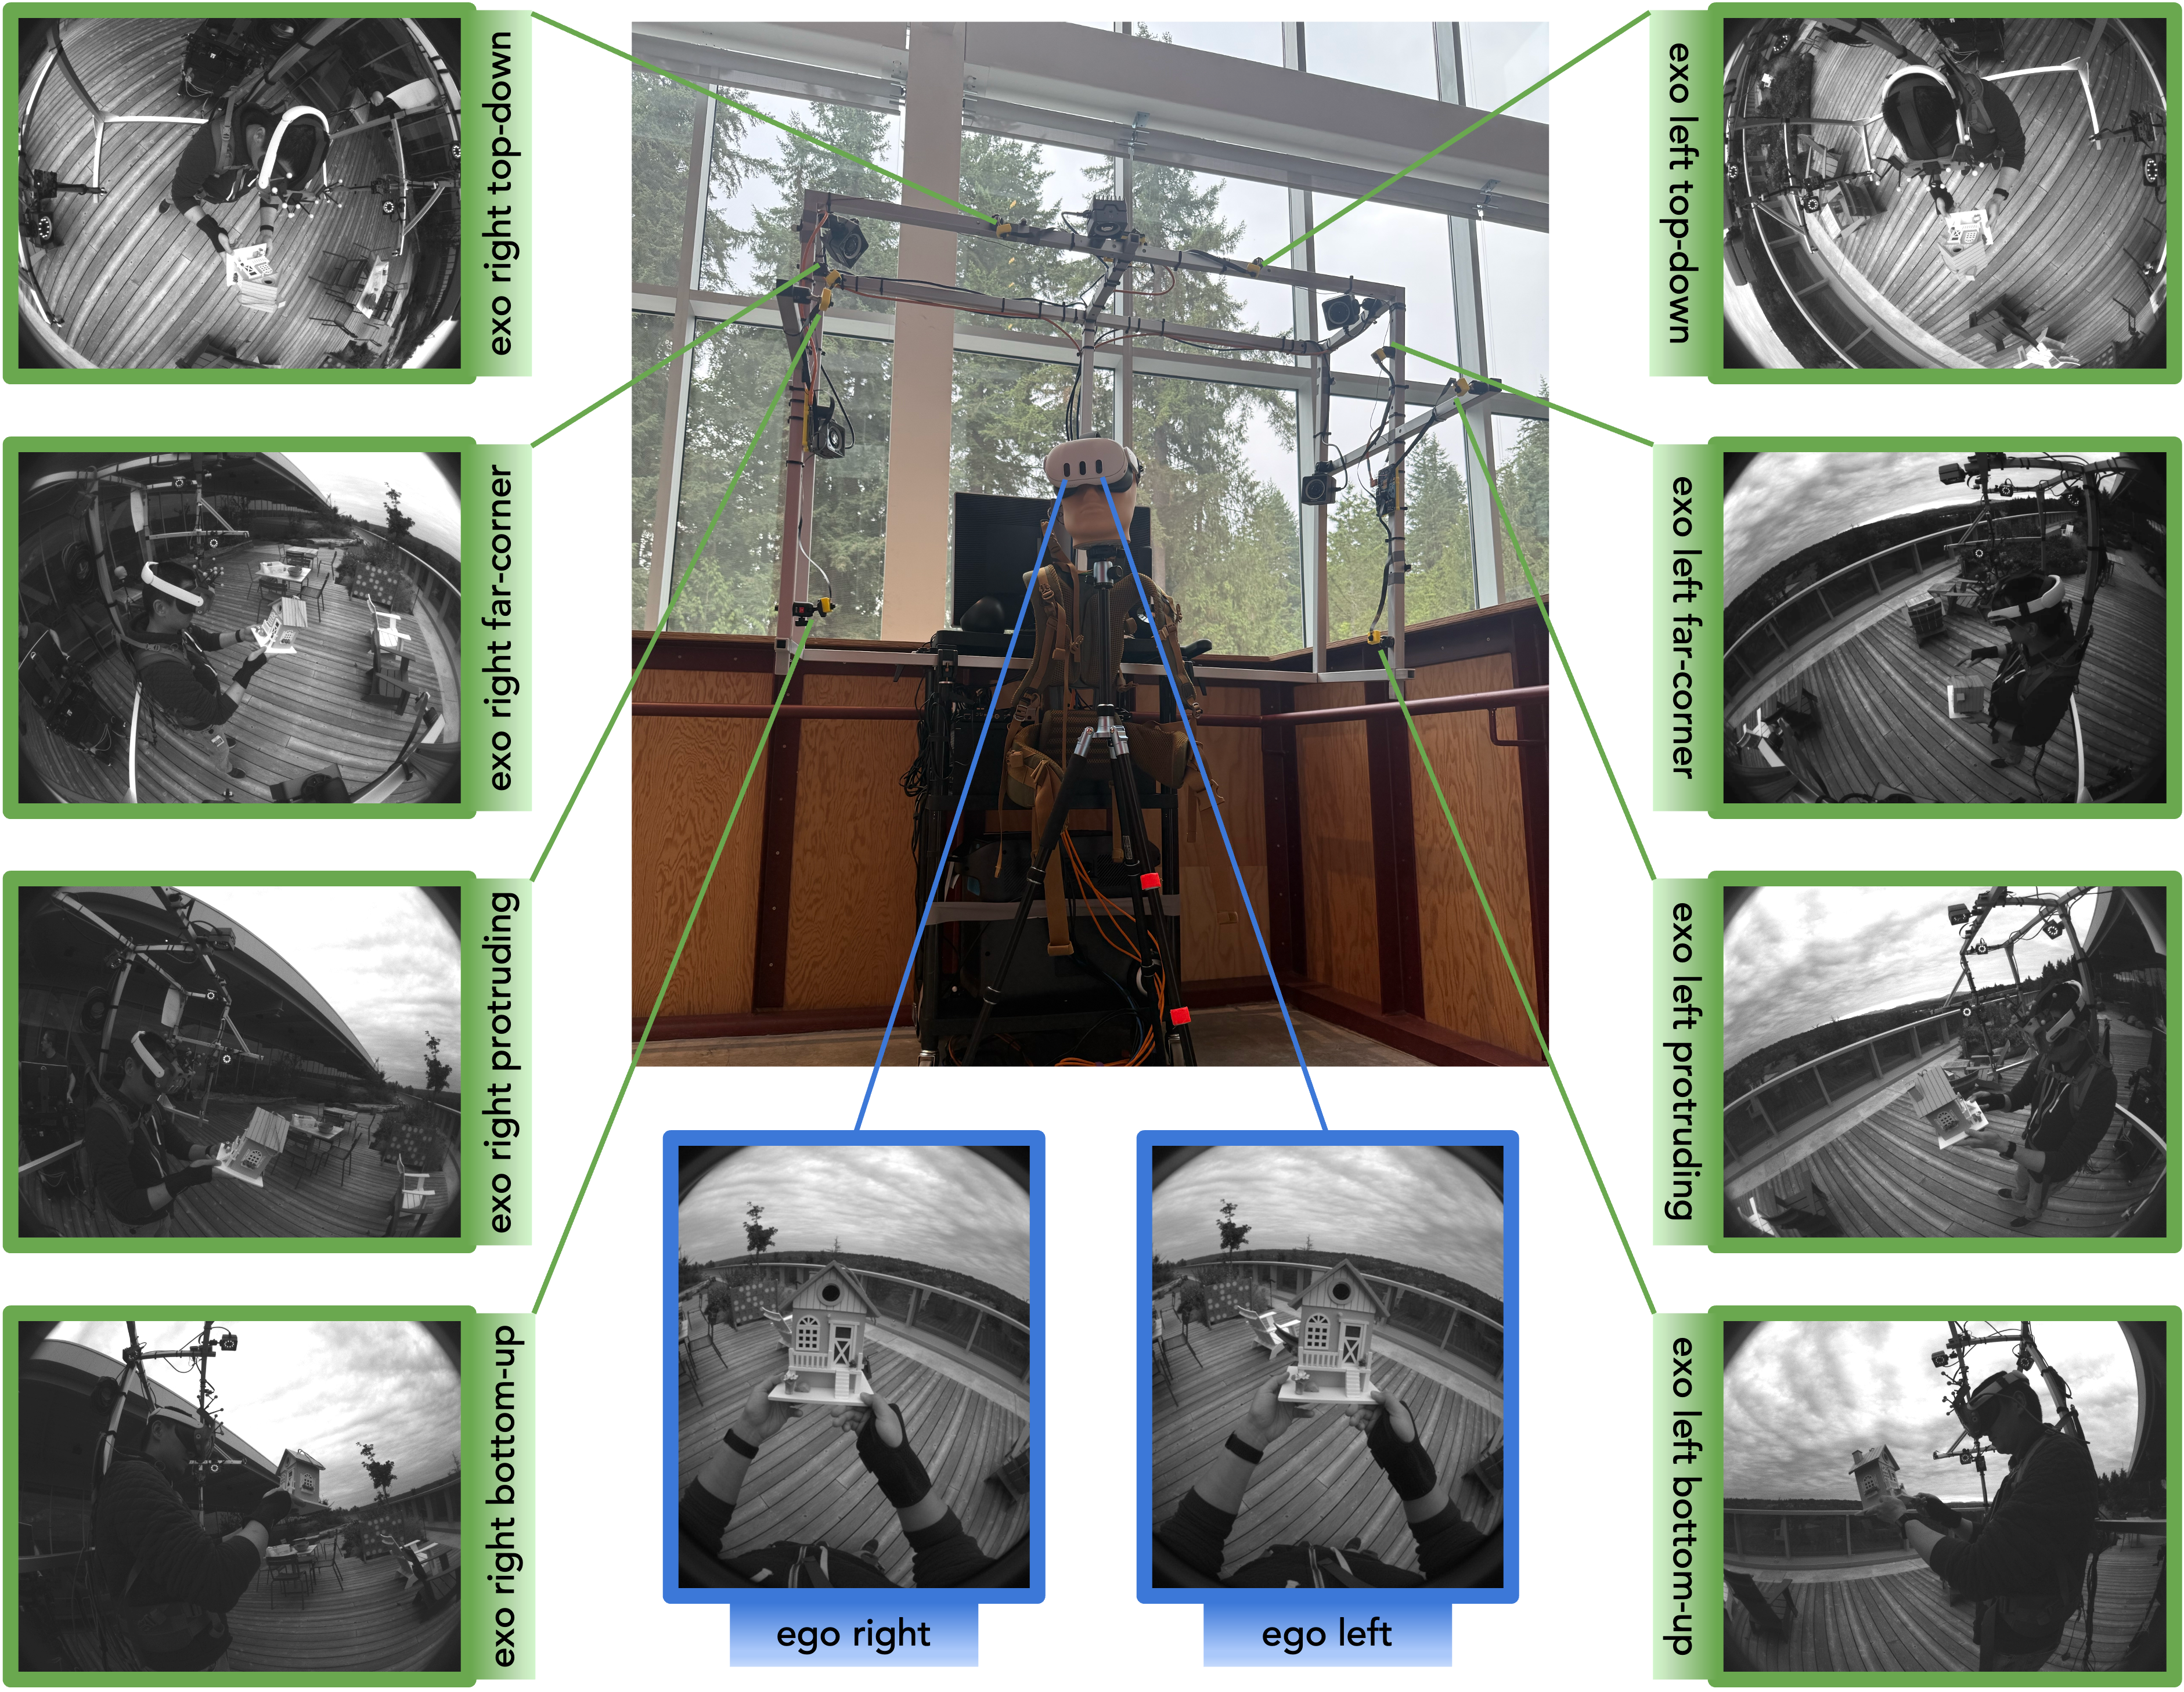
\includegraphics[width=.82\textwidth]{figures/SuppMat_Rig.png}%
    \captionof{figure}{
    \textbf{SHOW3D mobile capture setup.} The rig includes eight exocentric fisheye cameras (green) providing wide-baseline views from diverse angles, and two egocentric fisheye cameras (blue) mounted on the headset. This configuration enables full-surround imaging of hand–object interactions. We use monochrome cameras instead of RGB as they are more robust to illumination variability.
    }
    \label{fig:rig_details}
  \end{center}%
  \vspace{5pt}
}]


\section{Mobile Capture Rig Details}
Figure~\ref{fig:rig_details} depicts our mobile capture rig and example images captured by each camera.
All camera and MoCap data are streamed, via USB and Ethernet, to 
a high-performance desktop workstation placed on a rolling cart.
The specs of the workstation are:
AMD Ryzen Threadripper PRO 3995WX 64-core processor, 128GB RAM, and 30TB SSD storage.
We power the workstation with a 2048Wh portable power station, which supports up to three hours of continuous capture.

We employ five OptiTrack Prime 13W MoCap cameras for tracking the IR-reflective markers fixed to the top of the user-worn headset; the set of markers are tracked altogether as a rigid body. 
We use a custom solution to calibrate the MoCap system, the rig cameras, and the headset cameras all into a shared 3D space. Then, the per-frame extrinsics of the headset cameras can be  inferred via the 6DoF transform of the tracked rigid body, such that the 3D ground truth computed from rig cameras can be precisely projected into the headset cameras for every frame.

All of the monochrome fisheye cameras run an autoexposure policy in real-time, to adapt to variable lighting conditions. Headset cameras are controlled by Quest 3's on-device autoexposure algorithm, while for the rig cameras, our capture software enforces a target average intensity of 60 over the entire image.


\begin{figure}[t]
    \centering
    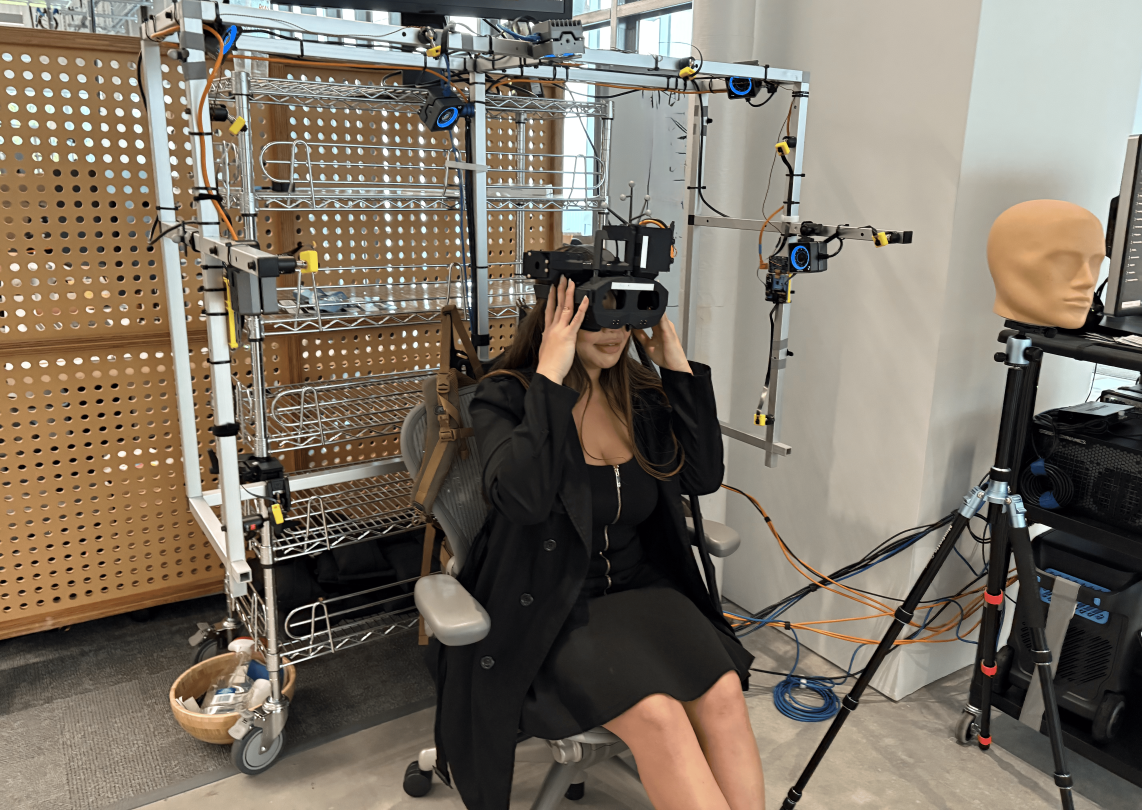
\includegraphics[width=.9\linewidth]{figures/sitting.png}
    \caption{\textbf{Stationary configuration for inclusive capture.} The rig can be mounted statically to allow for seated data collection. This setup eliminates the weight burden of the backpack, accommodating participants with limited mobility or physical endurance.}
    \label{fig:sitting_setup}
\end{figure}

\subsection{Inclusive Design via Stationary Configuration}

To ensure that our dataset captures a diverse range of participants, we designed our system to be adaptable to different physical needs. While the primary configuration is a wearable backpack, the rig can also be fixed to a rolling cart, with a chair placed inside so the participant assumes the same relative position as if wearing it (see Figure~\ref{fig:sitting_setup}).

This configuration allows participants to perform hand-object interactions while seated, completely removing the physical burden of carrying the backstrap rig on the body. This adaptation is critical for inclusivity, as it enables participation from individuals with limited physical endurance, mobility constraints, or those who would otherwise be unable to support the weight of the rig for extended periods. This way, we ensure that our data collection is accessible to, and representative of, a broader demographic.



\section{SHOW3D Dataset Details}

\begin{figure}[t]
    \centering
    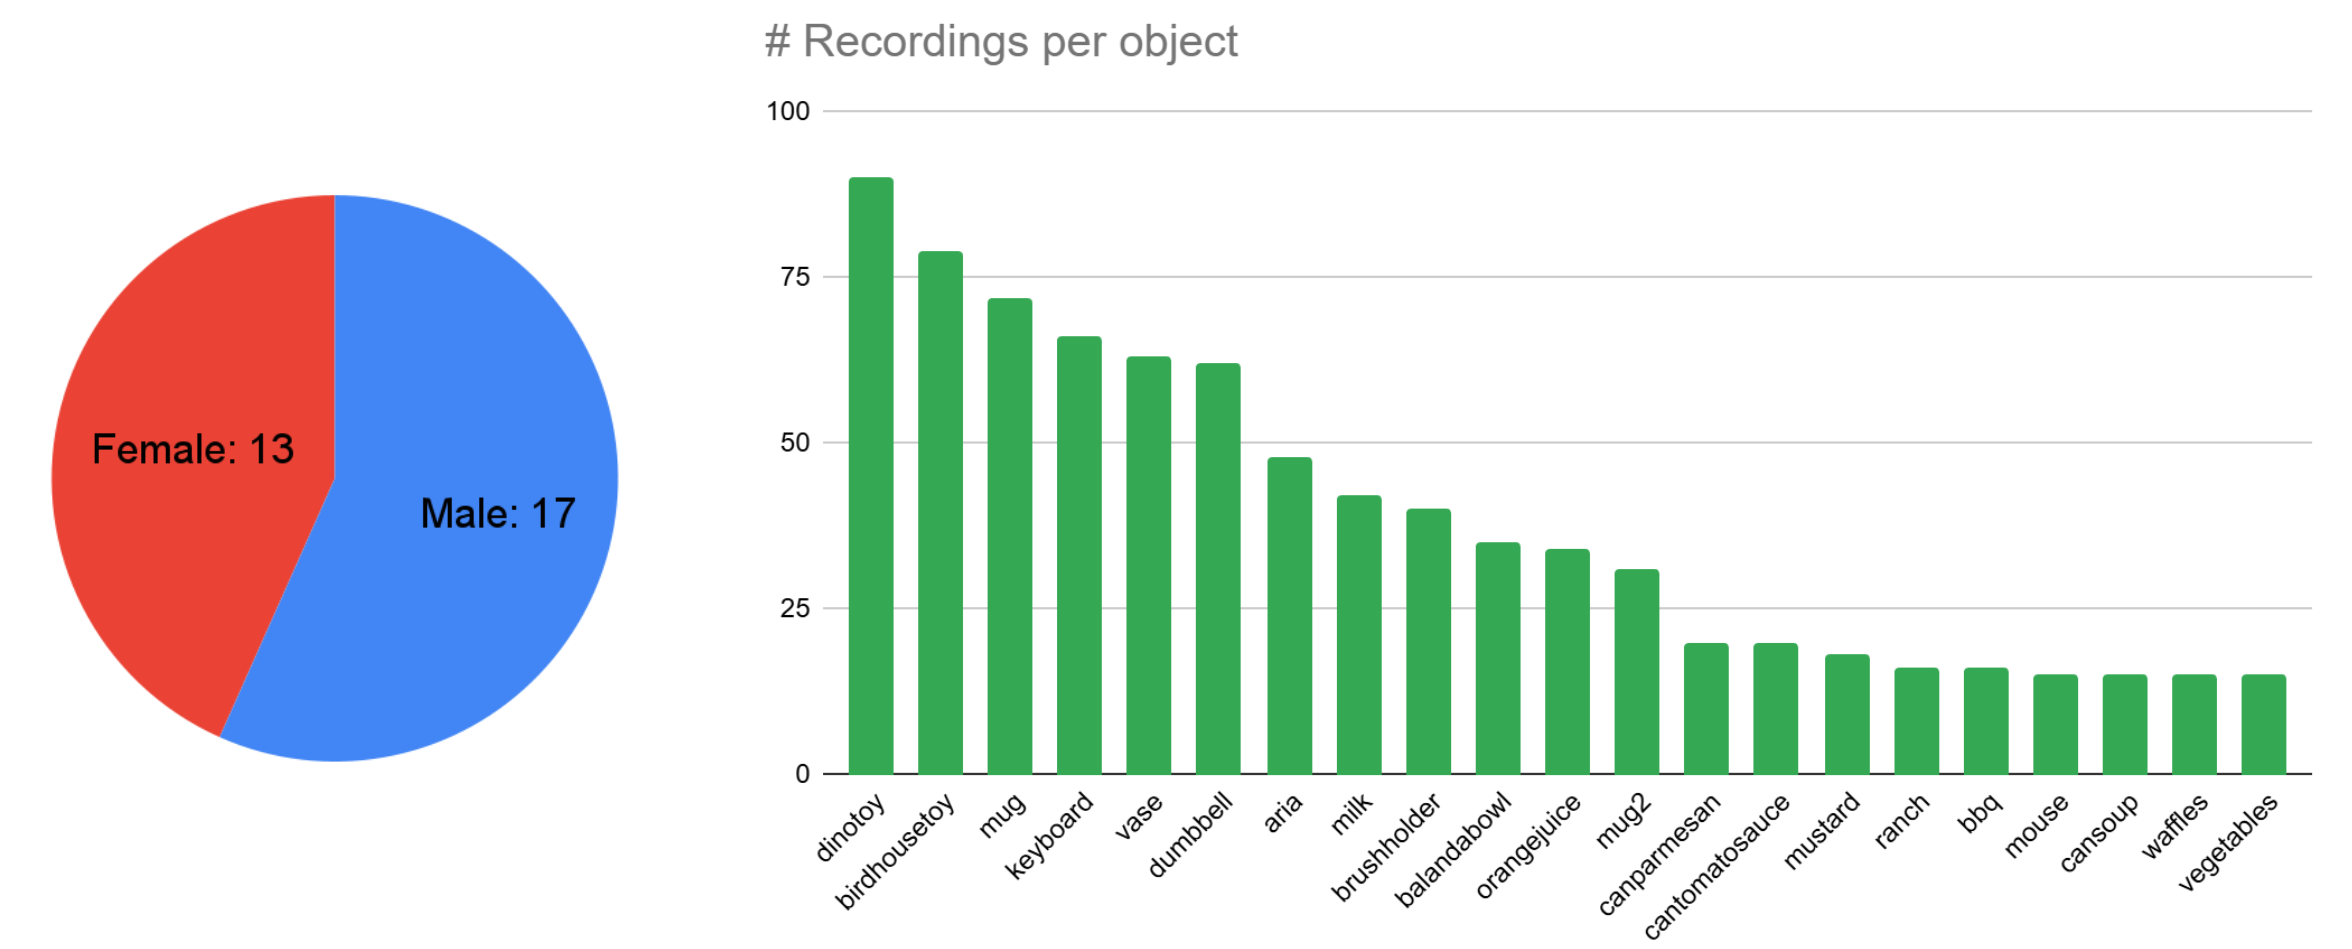
\includegraphics[width=\linewidth]{figures/dataset_stats.png}
    \caption{\textbf{SHOW3D dataset statistics.} 
    Left: participant distribution. 
    Right: number of recordings per each of the 21 objects.
    }
    \label{fig:dataset_stats}
\end{figure}

\customparagraph{Dataset Construction and Statistics.} 
We collected around 20 hours of synchronized ego-exo video data at 60Hz, resulting in 4.3M unique frames, or 43M unique images from all cameras. 
The dataset captures a large variety of indoor/outdoor environments, hand motions, and object interactions.
In a subset of around 2M frames, we captured hand-object interaction with a total of 21 objects procured from the list used in HOT3D~\cite{banerjee2025hot3d}.
The rest of the dataset feature bare-hand motion, hand-hand interaction, or hand-object interaction with other non-HOT3D objects that we currently do not have 3D scans for.

We recruited 38 human participants (24 male, 14 female) with a wide range of hand shapes and sizes.
All participants signed a form stating their consent for their collected data to be used for research purposes.
In addition, we employ a commercially available high-resolution optical scanning system to obtain a personalized hand model for each participant. The personalized model is a linear blend skinning mesh in UmeTrack~\cite{han2022umetrack} format, which can be fit to detected 3D keypoints via Inverse Kinematics.

\begin{figure}[t]
    \centering
    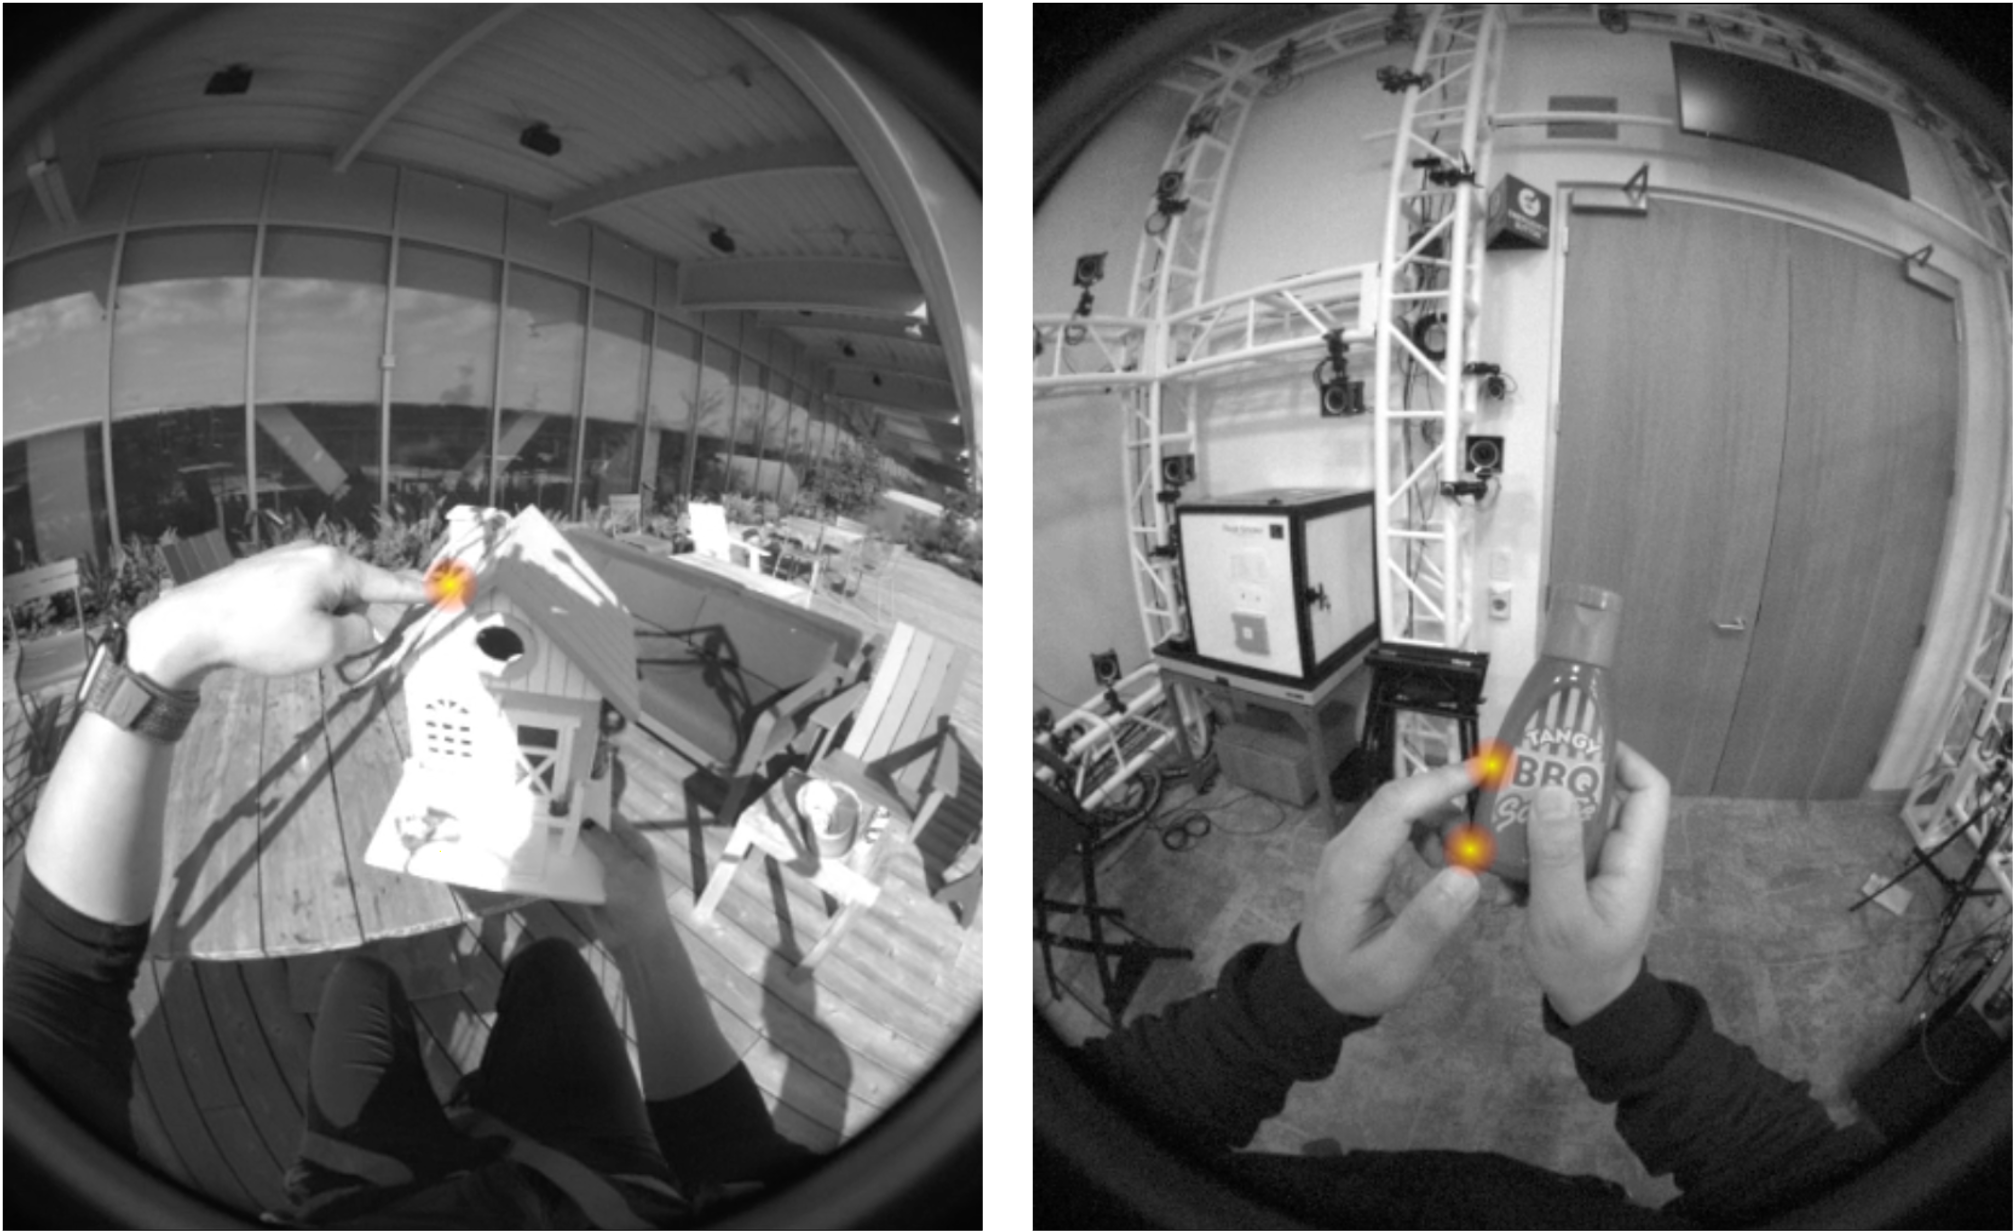
\includegraphics[width=\linewidth]{figures/contacts.png}
    \caption{\textbf{Examples of contact annotations.}  Egocentric frames from SHOW3D with annotated contact regions (yellow). For visual clarity, contact annotations are only shown between the left hand and the manipulated object.}
    \label{fig:left_contact}
\end{figure}


\customparagraph{2D Segmentation Masks.} 
We automatically generate 2D segmentation masks for both hands and objects by projecting the annotated 3D meshes into each camera view using the calibrated intrinsic parameters. We can further utilize the projected mask as a prompt for the Segment Anything Model (SAM 2)~\cite{ravi2024sam} to obtain high-quality, refined 2D segmentation masks suitable for training 2D vision tasks.

\customparagraph{Contact Regions.} 
Leveraging our precise mesh reconstructions, we generate detailed contact annotations by calculating the Euclidean distance from every vertex on the hand mesh to the nearest point on the object surface. Vertices with a distance below some threshold (e.g., 5mm) are labeled as contact points. This results in continuous, vertex-level contact maps (see Figure~\ref{fig:left_contact}) that capture the functional grasp regions during dynamic interactions. 


\section{3D Hand Annotation Quality}
\begin{figure}[t]
    \centering
    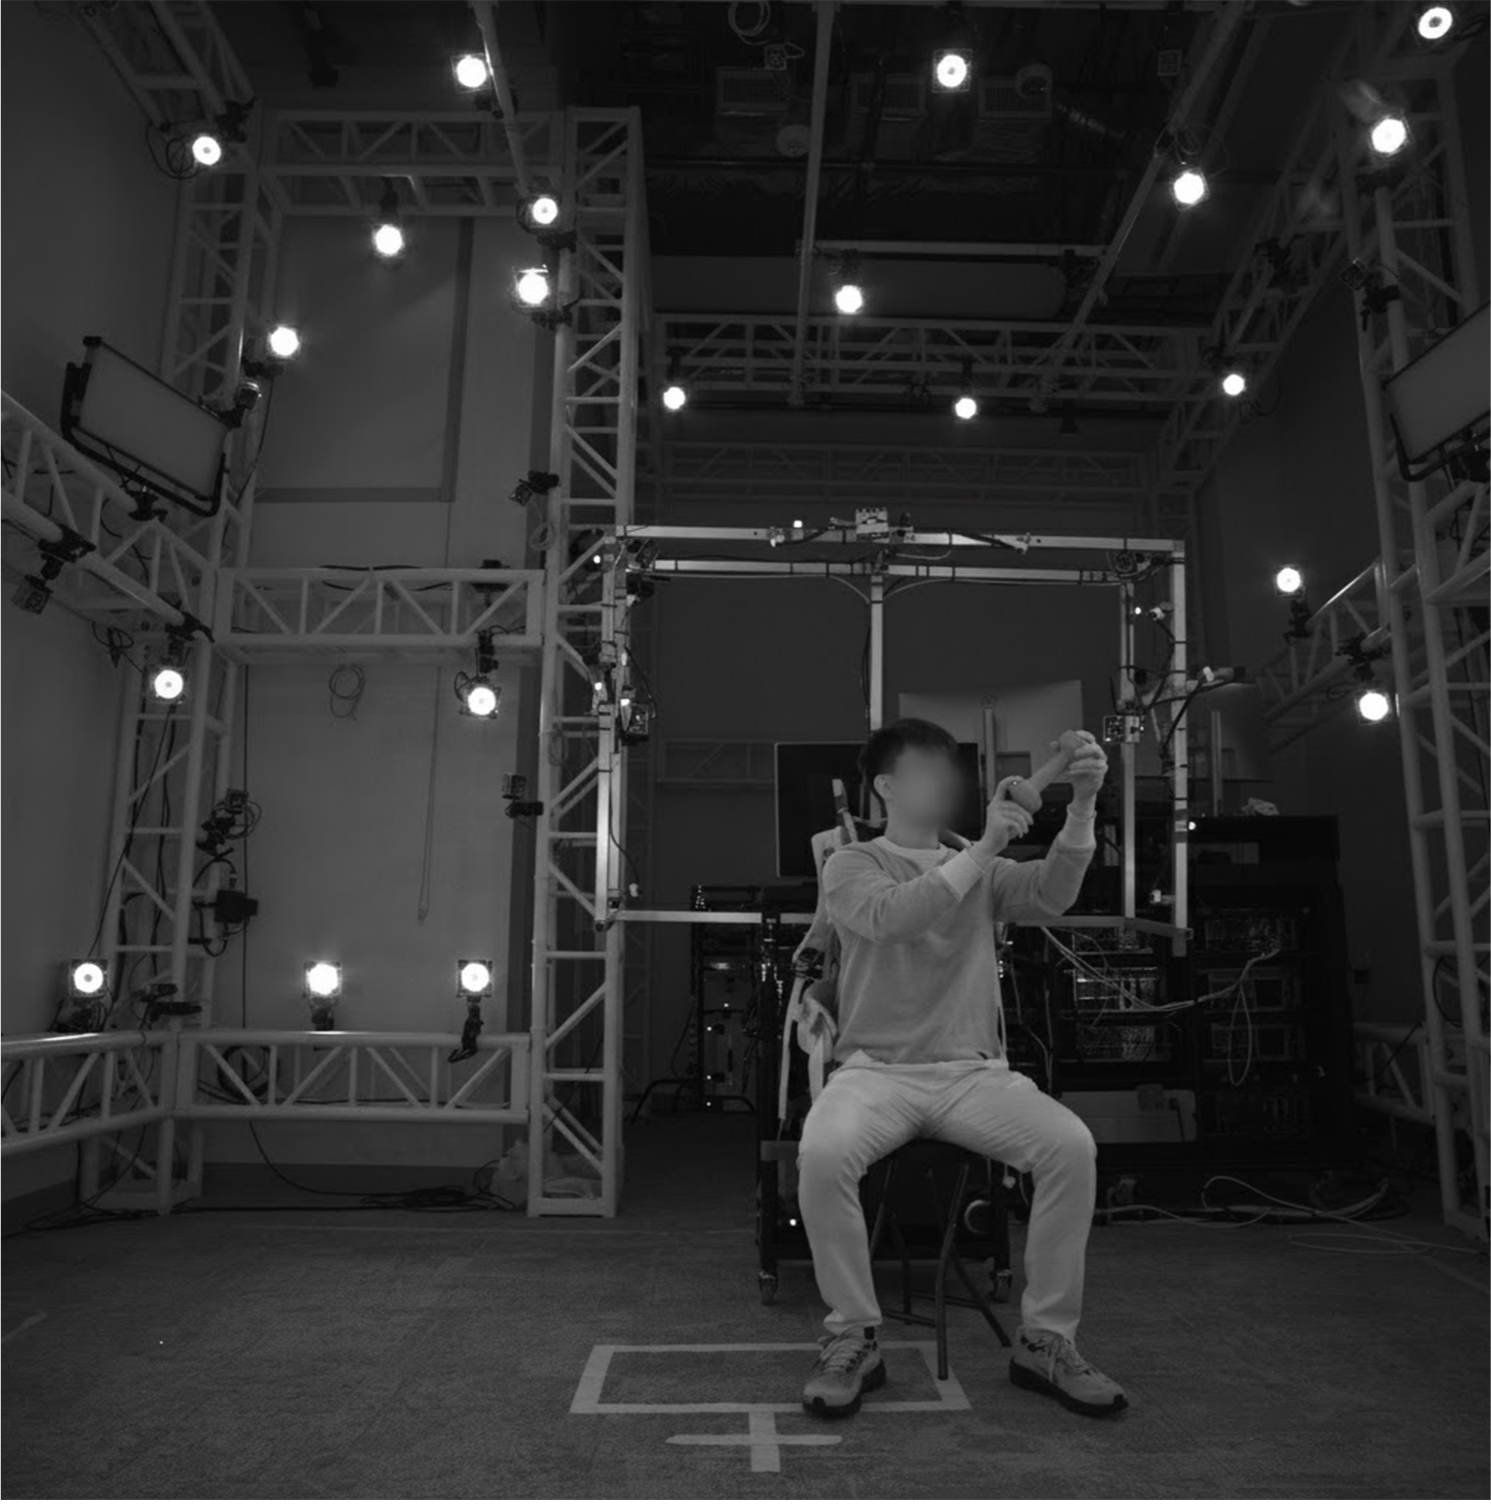
\includegraphics[width=0.9\linewidth]{figures/dome_blurred.png}
    \caption{\textbf{Simultaneous rig--dome capture for ground truth validation.} 
    To evaluate the accuracy of our mobile annotation pipeline, we captured sequences where the subject wears our mobile rig inside a high-fidelity stationary multi-camera dome. 
    This allows for a direct comparison between our mobile-rig-derived annotations and the dome-derived ``gold standard.''}
    \label{fig:dome_capture}
\end{figure}


To validate the accuracy of the 3D hand poses generated by our mobile rig via our ego-exo pipeline (see Figure 3 of the main paper, and Figure~\ref{fig:hand_gt_pipeline}), we compare our automated annotations against two distinct ``gold standard'' sources: a stationary multi-camera studio system and human manual annotation, that we select over other choices of sensor and modality~\cite{kim2009multi, sun20213drimr, xia2023quadric, alexiadis2016integrated, rim2025protodepth}.


\customparagraph{Experimental Setup.}
We define the two evaluation protocols as follows:
\begin{itemize}
    \item \textbf{Dome} (in-studio validation): We engaged a participant to wear our mobile rig \emph{inside} a large-scale, stationary multi-camera dome system equipped with 30 calibrated cameras (see Figure~\ref{fig:dome_capture}). The Dome system provides high-precision automated 3D keypoints via massive multi-view triangulation, serving as a proxy for human-annotated ground truth in a controlled environment. 
    To align the coordinate systems, we attached reflective markers to the mobile rig and utilized the dome's infrared motion capture system to calibrate the rig into the dome's 3D space.
    All data feeds—from both the rig and dome cameras—are synchronized with high precision.
    \item \textbf{Manual} (in-the-wild validation): To validate performance in realistic outdoor conditions where the Dome is unavailable, we sampled a subset of frames from our in-the-wild captures. Crowd-sourced annotators manually labeled 2D keypoints on all available camera views. We then obtained 3D ground truth via robust RANSAC-based triangulation of these manual 2D labels.
\end{itemize}


\begin{table}[t]
\centering
\small
\resizebox{\columnwidth}{!}{%
\begin{tabular}{c l c c}
\toprule
& & \multicolumn{2}{c}{\textbf{MPJPE (mm)}} \\
\cmidrule(lr){3-4}
\textbf{Reference} & \textbf{Category} & \textbf{Median}$\downarrow$ & \textbf{P90}$\downarrow$ \\
\midrule
\multirow{3}{*}{Dome}
  & No interactions          & 6.28 & 7.31 \\
  & Hand–hand interaction    & 7.46 & 8.95 \\
  & Hand–object interaction  & 7.90 & 12.53 \\
\midrule
\multirow{3}{*}{Manual (in the wild)}
  & No interactions          & 5.65 & 12.35 \\
  & Hand–hand interaction    & 6.03 & 14.63 \\
  & Hand–object interaction  & 6.36 & 16.48 \\
\bottomrule
\end{tabular}
}% end resizebox
\caption{Quantitative evaluation of our ground-truth hand annotations against two references: a high-coverage 30-camera dome (\textbf{Dome}) and manual annotations (\textbf{Manual}). We report median and 90th percentile per-frame MPJPE (mm).}
\label{tab:gt_evaluation}
\end{table}

\begin{figure}[t]
    \centering
    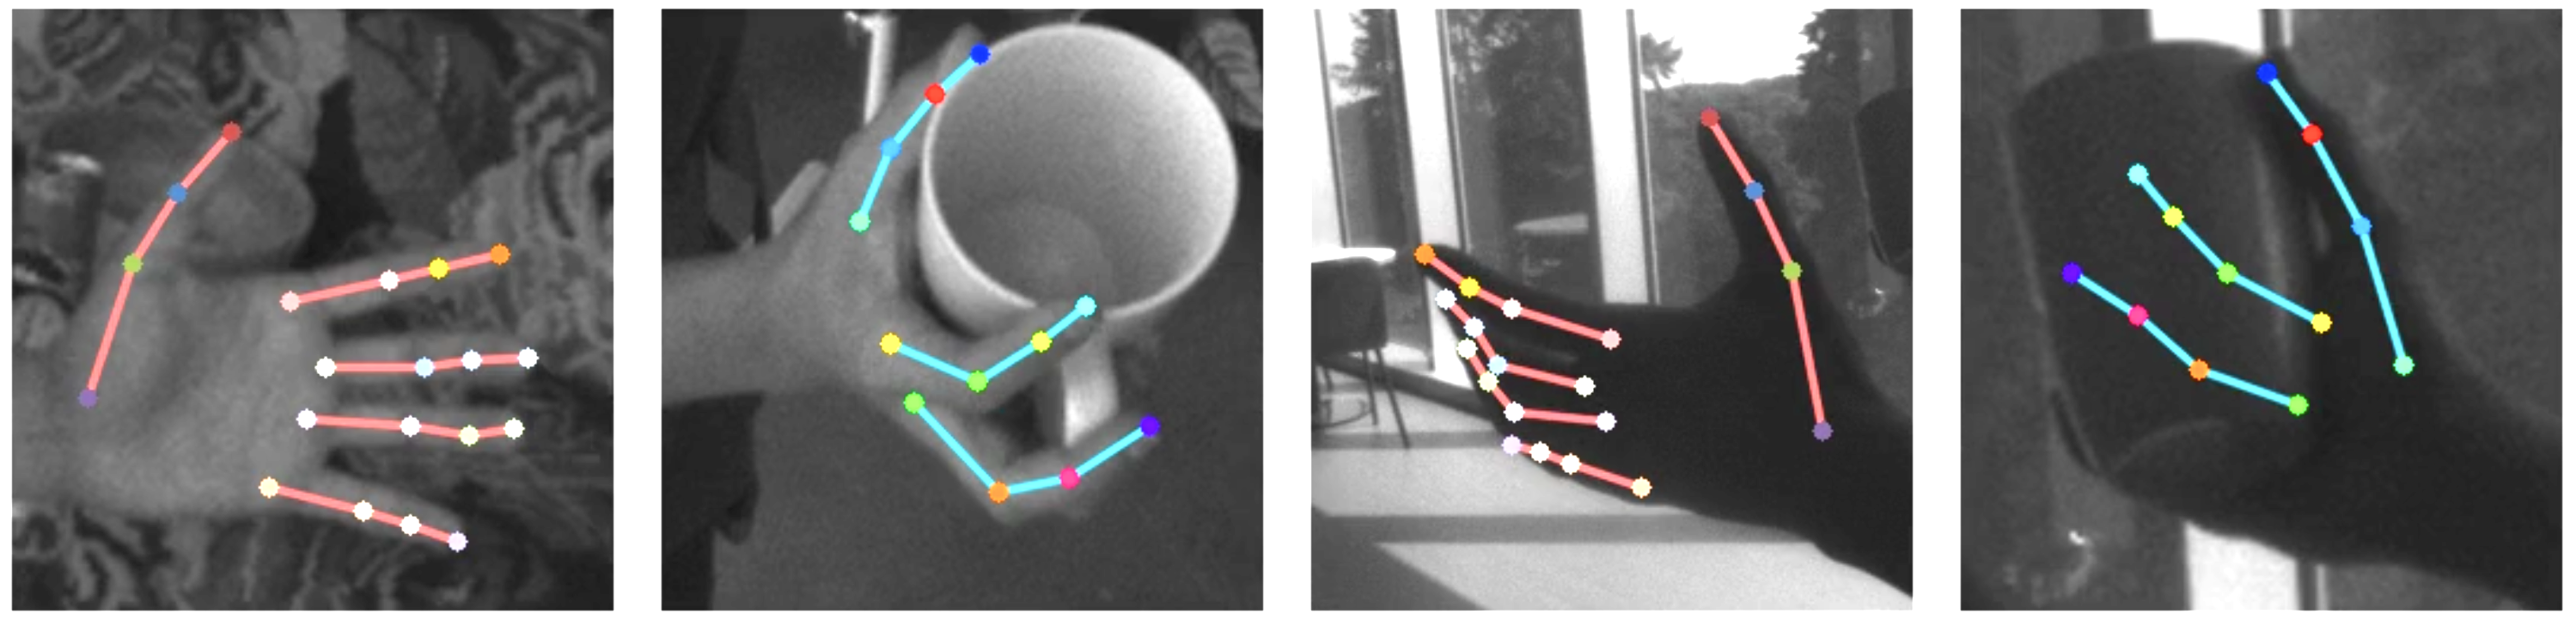
\includegraphics[width=\linewidth]{figures/manual_annotation.png}
    \caption{\textbf{Examples of manually annotated hand keypoints.} 
    Orange: left hand, blue: right hand. Note that the annotators are instructed to annotate only the keypoints that they have high confidence for.
    During evaluation, we only evaluate against annotated keypoints that have valid 3D triangulation.
    }
    \label{fig:manual_annotation}
\end{figure}


\customparagraph{Results and Analysis.}
Table~\ref{tab:gt_evaluation} reports the median and 90th percentile (P90) Mean Per-Joint Position Error (MPJPE) across three interaction complexity levels.

We observe that the \textbf{Manual} reference yields a lower median error than the \textbf{Dome} (e.g., 6.36mm vs. 7.90mm for hand-object interactions), but a higher P90 error (16.48mm vs. 12.53mm). 
We attribute this P90 discrepancy to the independence of the ground-truth generation methods. The Dome system relies on a multi-view algorithmic pipeline (automated keypoint detection and triangulation) that is methodologically similar to our own ego-exo pipeline. Consequently, the Dome and our system likely share similar failure modes—such as occlusion patterns or challenging lighting conditions—resulting in correlated errors that artificially dampen the P90 values. 
In contrast, human annotators provide a truly independent ground truth. They do not suffer from algorithmic biases and can accurately label challenging views that automated detectors might miss or misinterpret. Therefore, the Manual evaluation is a more rigorous ``stress test,'' exposing the true outlier failure cases of our triangulation-based approach that remain hidden when comparing against another automated system.

Importantly, across both evaluation protocols and all interaction types, our pipeline consistently achieves \textbf{sub-centimeter median accuracy}. Even in the most challenging scenario—hand-object interaction—our median error remains below 8mm against the Dome and below 7mm against manual annotation. 
These results confirm that our mobile, markerless capture system generates 3D ground truth of sufficient quality to train downstream egocentric perception models~\cite{han2020megatrack, han2022umetrack, pavlakos2024reconstructing, zhang2016learning, yang2024mlphand, prakash20243d, fan2023arctic}, successfully bridging the gap between studio fidelity and in-the-wild diversity.


\begin{figure*}[ht]
    \centering
    \begin{minipage}[b]{0.672\textwidth}
        \begin{subfigure}[b]{\textwidth}
            \centering
            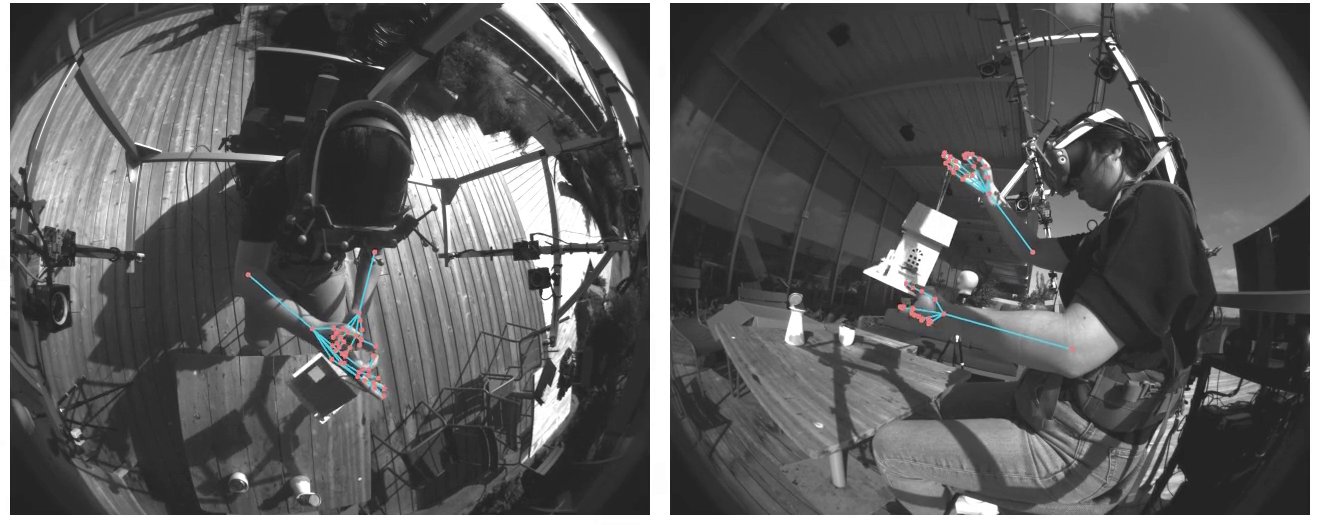
\includegraphics[width=\textwidth]{figures/hands_sapiens.png}
            \caption{Triangulated Sapiens keypoints: hand joints and forearm.}
            \label{fig:subfig1}
        \end{subfigure}
        \vspace{0.02\textwidth}
        \begin{subfigure}[b]{\textwidth}
            \centering
            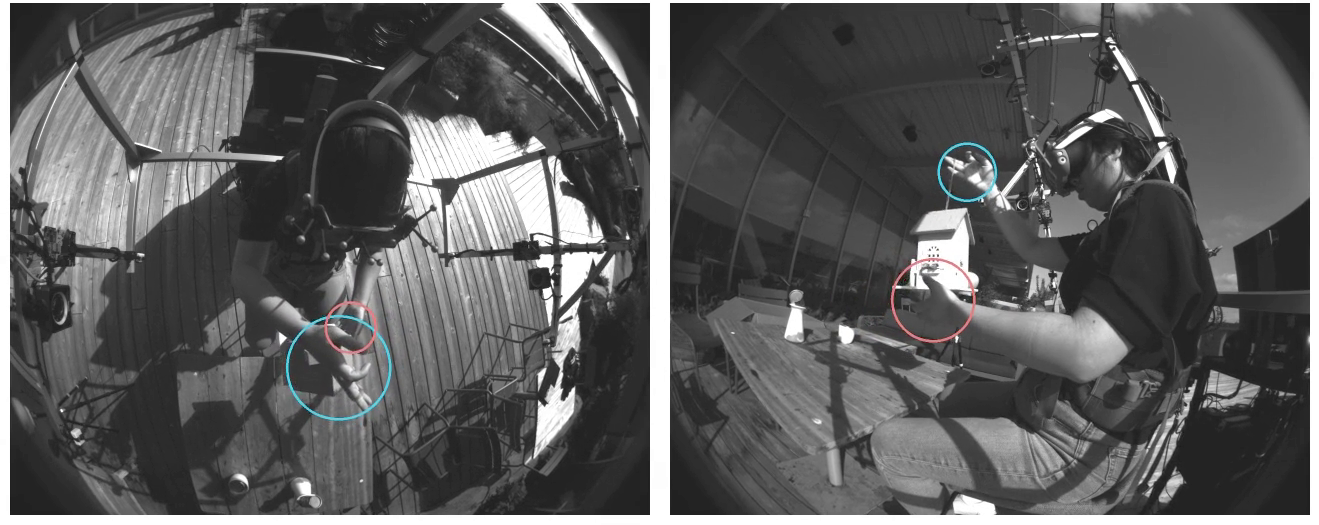
\includegraphics[width=\textwidth]{figures/hands_crop.png}
            \caption{Inferred crop regions for both hands.}
            \label{fig:subfig2}
        \end{subfigure}
    \end{minipage}
    \hfill
    \begin{minipage}[b]{0.285\textwidth}
        \begin{subfigure}[b]{\textwidth}
            \centering
            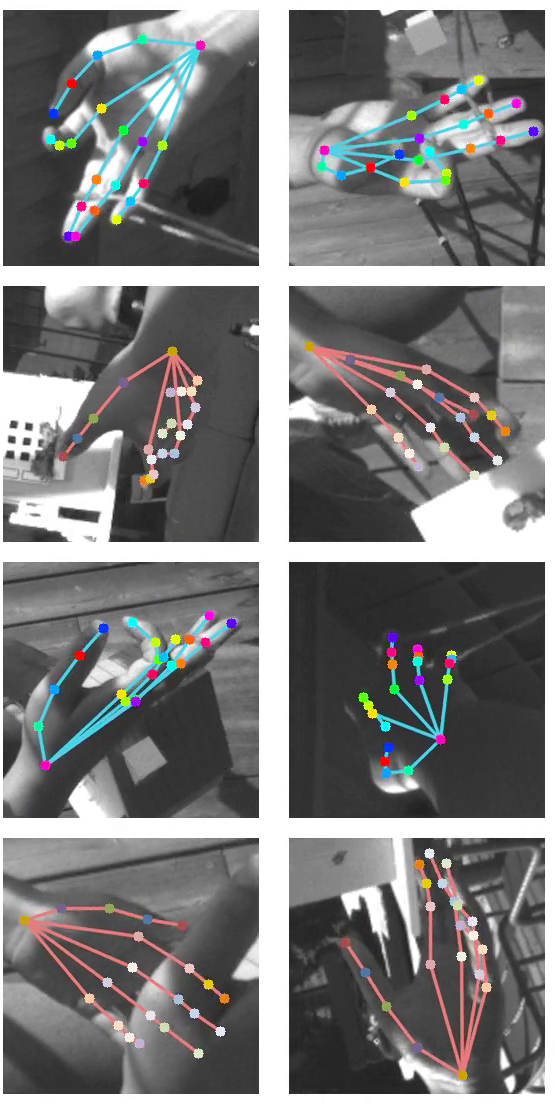
\includegraphics[width=\textwidth]{figures/hands_handsy42.png}
            \caption{Final hand keypoint detections. Orange: left hand, Blue: right hand.}
            \label{fig:subfig3}
        \end{subfigure}
        \vspace{-15pt}
    \end{minipage}
    
    \caption{Our automated pipeline for 3D hand keypoint annotation. (a) Sapiens keypoints: we use the triangulated hand and forearm keypoints to define crop regions for hands. 
    (b) Crop regions are used to generate 256x256 perspective crops \cite{han2022umetrack} for both hands.
    (c) We apply InterNet~\cite{Moon_2020_ECCV_InterHand2.6M} on the perspective crops, and fuse them with the initial Sapiens detections to obtain final 3D hand keypoints.
    }
    \label{fig:hand_gt_pipeline}
\end{figure*}

\section{6DoF Object Annotation Quality}

To quantitatively evaluate our object pose annotations, we attach optical markers to 5 selected objects and track them using a MoCap system while they are being manipulated by hands.
We evaluate our GT object poses against the MoCap object poses (``gold standard'') in Table~\ref{tab:obj_annotation} by comparing the yield (\% of annotated frames), translation error (TE), and rotation error (RE).
The yield and accuracy of our GT object poses are generally very high, except for {\small \texttt{bottle\_bbq}}, which is a smaller and thus harder to detect object.
These results make SHOW3D the first HOI dataset to quantitatively evaluate both its 3D hand pose and 6DoF object pose annotations against independent references.
\begin{table}[h]
\footnotesize
\centering
\vspace{-6pt}
\resizebox{\columnwidth}{!}{%
\begin{tabular}{c c c c}
\toprule
Object & Yield (\%) & P50 TE (mm)$\downarrow$ & P50 RE (deg)$\downarrow$ \\
\midrule
birdhouse\_toy  & 89.5 & 3.51 & 1.73 \\
carton\_oj  & 92.6 & 3.20 & 1.23 \\
dumbbell\_5lb  & 86.1 & 1.53 & 1.63 \\
aria\_small  & 77.3 & 2.79 & 1.81 \\
bottle\_bbq  & 53.5 & 2.60 & 5.77 \\
\bottomrule
\end{tabular}
\vspace{-40pt}
}% end resizebox
\caption{Quantitative evaluation of our ground-truth object annotations against MoCap-derived poses as an independent reference.}
\label{tab:obj_annotation}
\end{table}


\section{Ground Truth Pipeline Details}
As mentioned in Section~3.2 of the main paper, we use a multi-stage ego-exo pipeline to obtain 3D hand annotations. 
We illustrate this pipline in detail with Figure~\ref{fig:hand_gt_pipeline}.

While the Sapiens~\cite{khirodkar2024sapiens} keypoint model exhibits strong generalization on in-the-wild images, we observe that its hand keypoint quality is often suboptimal, likely because the backbone's feature resolution is insufficient for recognizing finer details. 
Our insight is that applying a dedicated hand keypoint detector on cropped and resized images helps to improve performance; note that cropping can remove background variations to a large extent, resulting in an easier detection problem.
On the other hand, the initial Sapiens keypoint detections are robust enough for defining rough crop regions for both hands, even under heavy occlusion during object interaction.

\begin{table*}[!t]
\centering
\resizebox{\textwidth}{!}{%
\begin{tabular}{c l *{13}{c} c}
\toprule
\shortstack{Frames\\ahead} & &
\rotatebox{45}{pouring in} & \rotatebox{45}{picking up} & \rotatebox{45}{pouring out} &
\rotatebox{45}{opening} & \rotatebox{45}{stirring} & \rotatebox{45}{placing down} &
\rotatebox{45}{raising} & \rotatebox{45}{shaking} & \rotatebox{45}{tapping} &
\rotatebox{45}{washing} & \rotatebox{45}{checking} & \rotatebox{45}{inspecting} &
\rotatebox{45}{moving} &
Mean \\
\midrule

% ---------- 30-FRAME BLOCK ----------
\multirow{3}{*}{30} & w/o text
 & 45.8 & 35.7 & 56.1 & 30.4 & 49.9 & 38.2 & 31.0 & 33.8 & 29.3 & 64.5 & 46.8 & 61.9 & \textbf{56.2}
 & 44.6 \\
 & w/ text
 & \textbf{28.3} & \textbf{23.6} & \textbf{37.3} & \textbf{20.5} & \textbf{35.0} & \textbf{29.4} & \textbf{24.5} & \textbf{27.5} & \textbf{26.1} & \textbf{59.7} & \textbf{44.9} & \textbf{61.2} & 59.1
 & \textbf{36.7} \\
 \hdashline \\[-2ex]
 & Improv.
 & 38.2\% & 33.9\% & 33.5\% & 32.6\% & 29.9\% & 23.0\% & 21.0\% & 18.6\% & 10.9\% & 7.4\% & 4.1\% & 1.1\% & -5.2\%
 & 17.7\% \\
\midrule

% ---------- 60-FRAME BLOCK ----------
\multirow{3}{*}{60} & w/o text
 & 53.1 & 41.8 & 60.6 & 34.4 & 48.4 & 40.1 & 37.8 & 40.9 & \textbf{29.9} & \textbf{71.6} & 55.7 & \textbf{63.8} & 69.7
 & 49.8 \\
 & w/ text
 & \textbf{35.4} & \textbf{26.7} & \textbf{42.8} & \textbf{22.6} & \textbf{40.2} & \textbf{31.9} & \textbf{25.7} & \textbf{30.7} & 32.2 & 73.6 & \textbf{51.2} & 63.9 & \textbf{68.6}
 & \textbf{42.0} \\
 \hdashline \\[-2ex]
 & Improv.
 & 33.3\% & 36.1\% & 29.4\% & 34.3\% & 16.9\% & 20.4\% & 32.0\% & 24.9\% & -7.7\% & -2.8\% & 8.1\% & -0.2\% & 1.6\%
 & 15.8\% \\
\bottomrule
\end{tabular}%
}
\caption{Per-verb evaluation of text-driven 6DoF object pose forecasting, for a selected set of verbs. 
Reported are translation errors (mm, $\downarrow$) and the relative percentage improvement provided by text conditioning. 
The results are sorted by improvement at 30 frames. 
Our method shows robust gains on predictable actions (\emph{pouring}, \emph{opening}), but has limited impact on ambiguous ones (\emph{moving}, \emph{inspecting}).}
\label{tab:interaction_field_verb}
\end{table*}

As described in the main paper, we fuse hand keypoint detections from Sapiens and InterNet~\cite{Moon_2020_ECCV_InterHand2.6M} via robust triangulation.
We assign  a real-valued confidence to each triangulated 3D keypoint: this confidence value can be used as  a weight on positional constraints in the subsequent Inverse Kinematics (IK) optimization, to adjust the contributions from individual keypoints.
Our confidence formulation, intuitively, rewards keypoints for having a larger inlier count and a lower reprojection error.
Specifically, given RANSAC inlier count threshold $i_\textrm{T}$ and 2D reprojection error threshold $e_\textrm{T}$, and a triangulated keypoint with observed inlier count $i$ and average reprojection error $e_\textrm{rep}$ over inlier views,
we define the confidence $C$ as follows:
\begin{align}
E_\textrm{rep} & = \frac{e_\textrm{T}-e_{\textrm{rep}}}{e_\textrm{T}}\in (0,1),\\
 C  & = \left(E_{\textrm{rep}}\right) ^{{\gamma}/{max\{1,i-i_\textrm{T}\}}}.
\end{align}

First, the fraction $E_\textrm{rep}$ is inversely related to the average reprojection error, and bounded within $(0,1)$.
Then, we reward higher inlier counts by raising $E_\textrm{rep}$ to a power smaller than 1, thus increasing the resulting confidence value towards 1.
The reward factor can be additionally controlled by a free parameter $\gamma>0$.

Finally, we assign a per-frame confidence value to each hand after solving IK. 
In downstream experiments, we threshold this per-hand confidence to determine valid frames; the threshold can vary depending on the task.
We use a Bayesian formulation to compute the per-hand confidence, based on the intuition that the final error in the hand pose is compounded from the errors in both keypoint detection and IK.
For each  hand, we simply take the product between 1) the average confidence of its associated keypoints, and 2) a term inversely proportional to the residual error from IK solving.


\section{Additional Results on Text-driven\\6DoF Object Pose Forecasting}

In Table 3 of the main paper, we demonstrate that text conditioning improves forecasting accuracy by 29\% and 25\% on average across all object categories for predicting 30 and 60 frames ahead, respectively. However, aggregating results by object potentially ignores the underlying mechanism of \emph{how} language aids forecasting. We hypothesize that the ``kinematic utility'' of a text caption is less dependent on the object itself (e.g., \emph{dumbbell} vs. \emph{keyboard}) and more on the specific interaction protocol (e.g., \emph{pouring} vs. \emph{inspecting}).

To investigate this, we reorganize our evaluation based on the interaction verb (identified and extracted from the full text description) rather than the object class. Table~\ref{tab:interaction_field_verb} presents the translation errors grouped by a subset of 13 distinct verbs present in SHOW3D text descriptions, sorted by the relative improvement provided by text conditioning in forecasting 6DoF object pose at the 30-frame horizon.


\begin{figure*}
  \begin{center}
    \captionsetup{type=figure}
    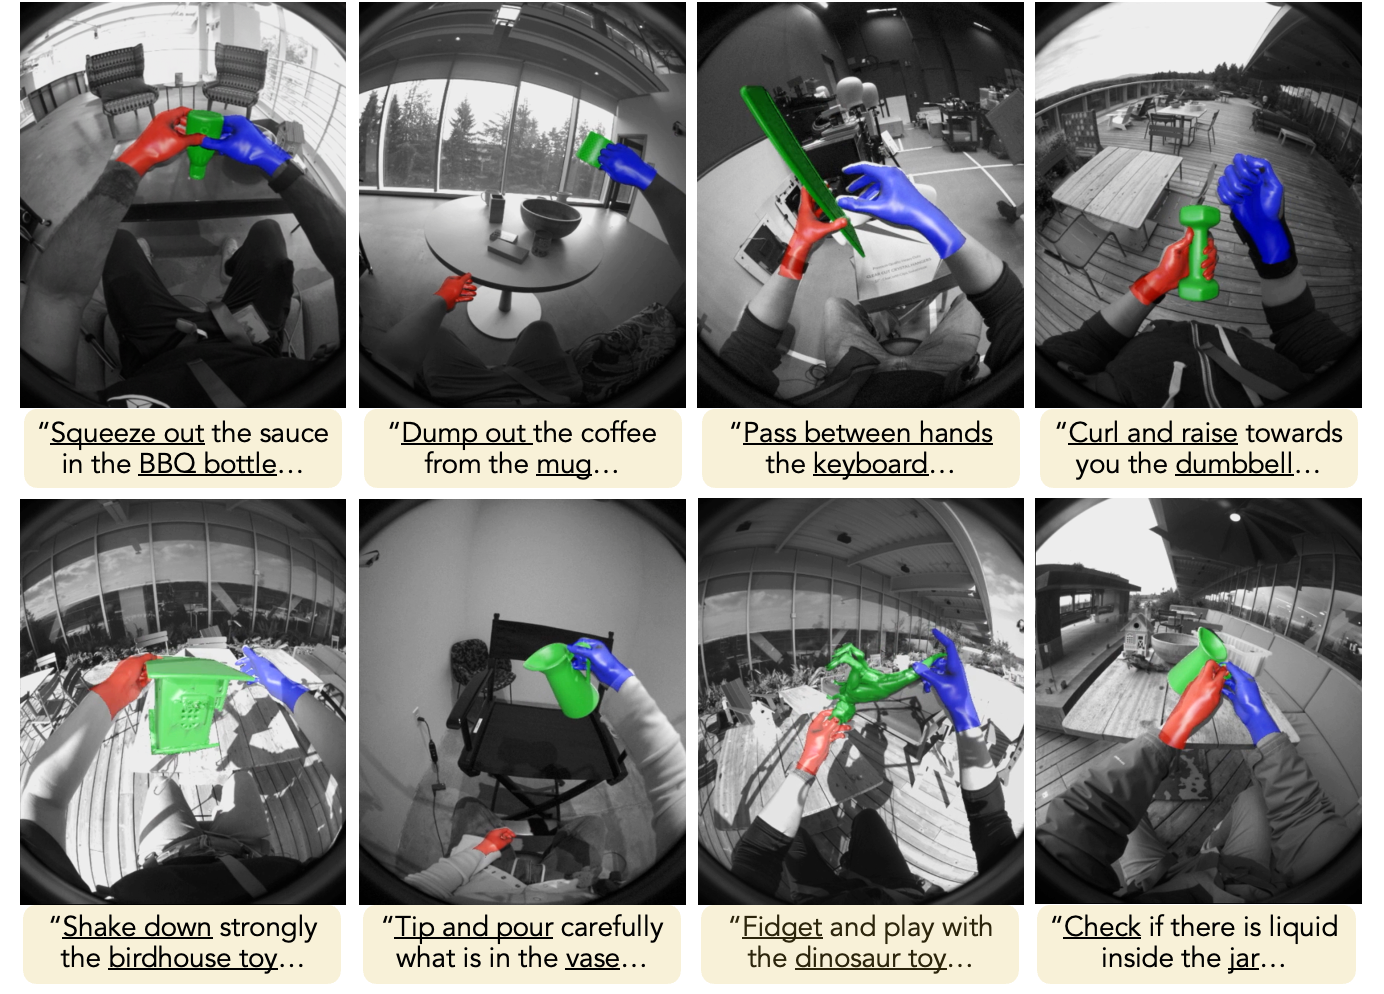
\includegraphics[width=.88\textwidth]{figures/SuppMat_Good1.png}%
    
    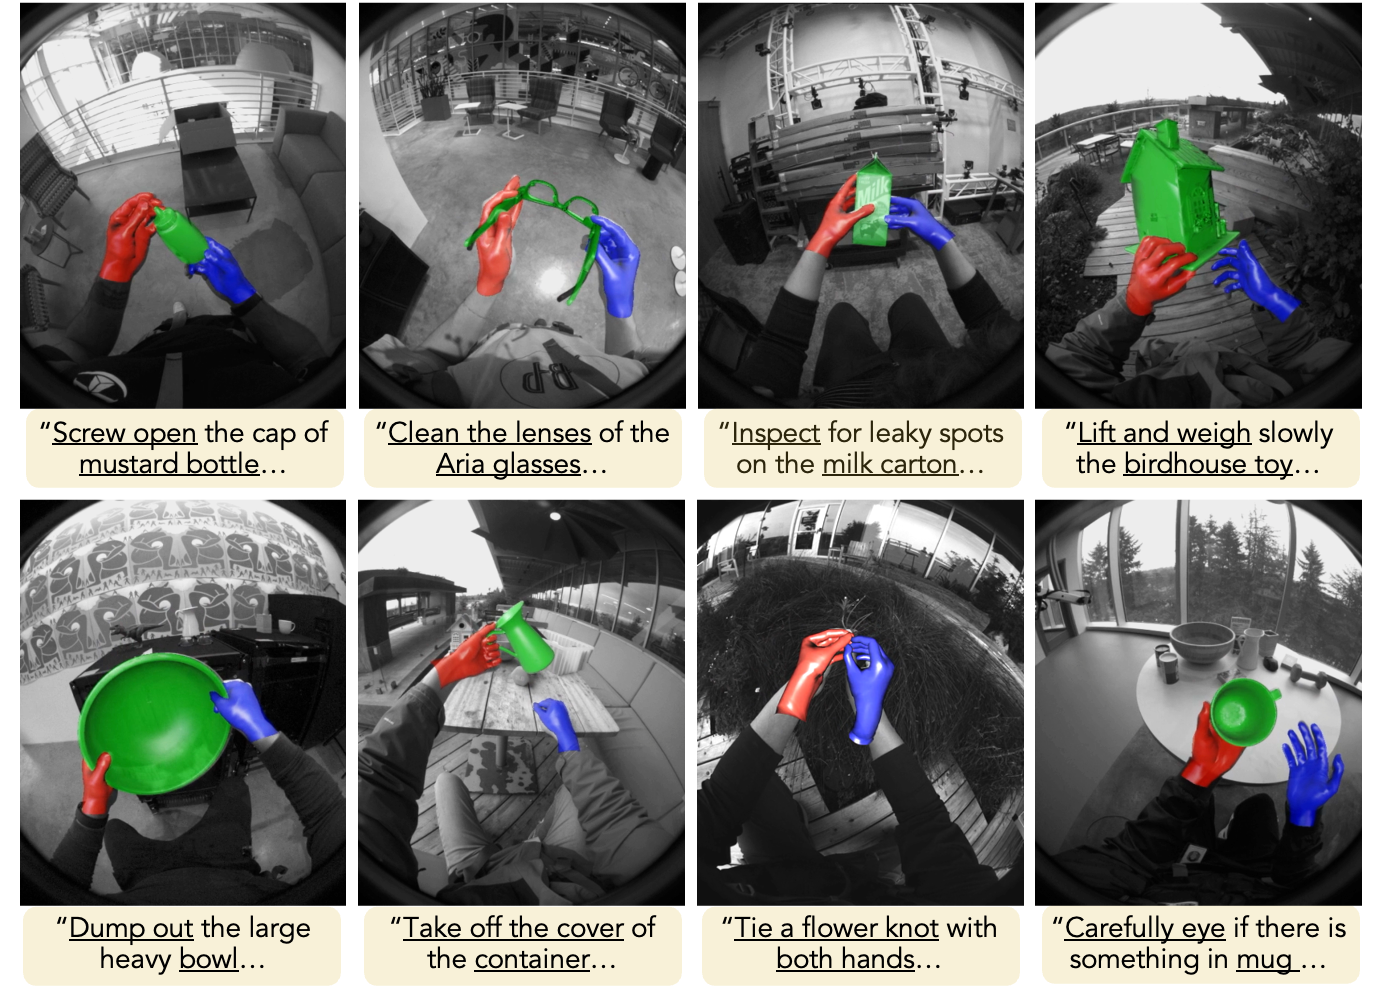
\includegraphics[width=.88\textwidth]{figures/SuppMat_Good2.png}%
    \vspace{-4pt}
    \captionof{figure}{
    Additional ground truth examples from SHOW3D: hand pose (red and blue), object pose (green), and text captions. 
    }
    \label{fig:suppmat_good1}
  \end{center}%
  \vspace{6pt}
\end{figure*}


\begin{figure}[t]
    \centering
    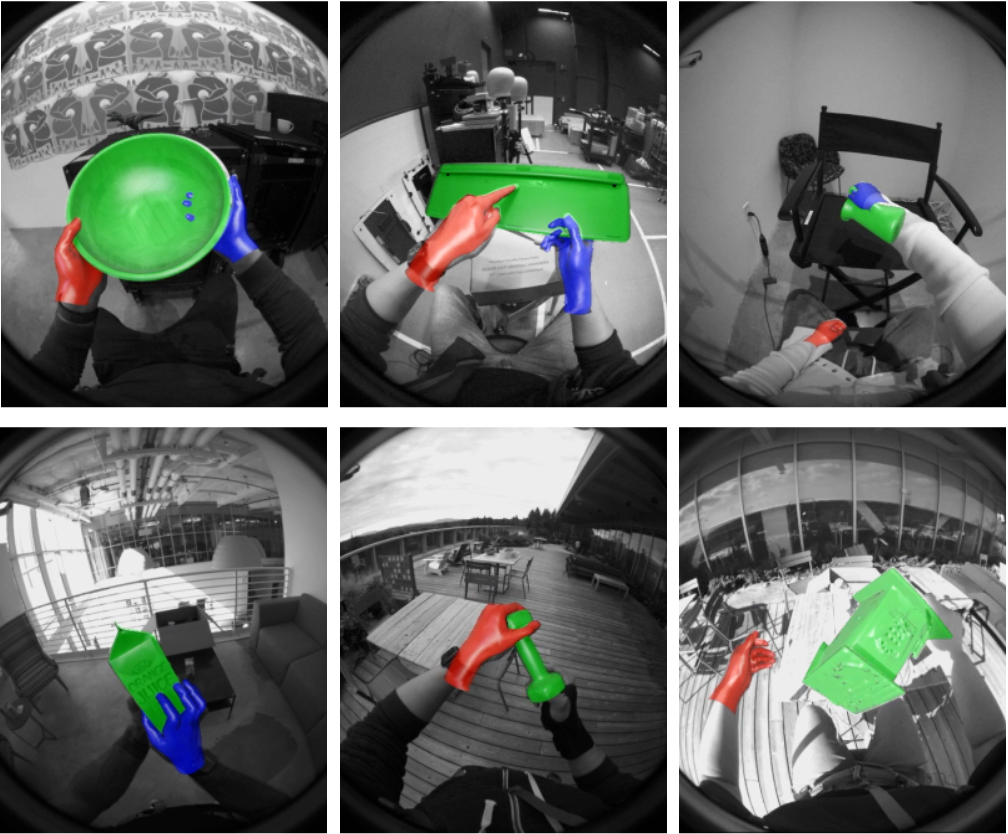
\includegraphics[width=\linewidth]{figures/SuppMat_Bad.png}
    \caption{\textbf{Hand annotation failure cases.} We visualize two common error modes in our automated annotation pipeline. 
    \textbf{Top row:} Examples of \textbf{inaccurate 3D pose estimation}. While all entities are successfully detected, minor errors in the estimated 6DoF pose result in physically implausible interpenetrations (clipping) between the hand and object meshes.
    \textbf{Bottom row:} Examples of \textbf{missed hand detections}. In scenarios with severe occlusion—where a hand is significantly obstructed by the object or the opposing hand—our pipeline occasionally fails to detect the occluded hand entirely.}
    \label{fig:failure_cases_general}
\end{figure}

\begin{figure}[t]
    \centering
    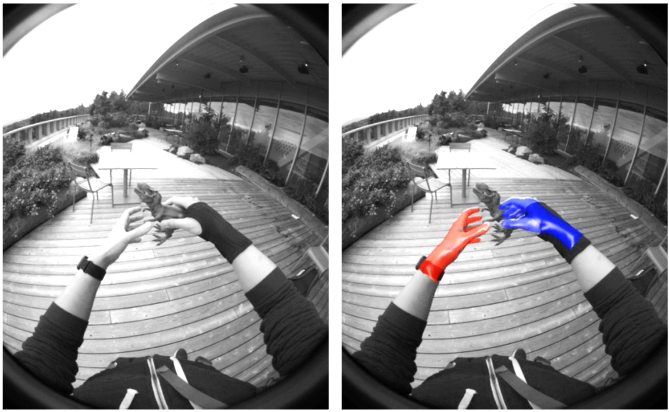
\includegraphics[width=\linewidth]{figures/SuppMat_Bad_noobj.png}
    \caption{\textbf{Object annotation failure case:} Missed object under severe occlusion and outdoor illumination.
    \textbf{Left:} The raw image from egocentric view.
    \textbf{Right:} The projected 3D hand meshes (red/blue) overlaying the image.
    Although the hands are correctly tracked, the object is not detected due to occlusion from both hands and strong outdoor lighting, and thus is entirely not tracked.}
    \label{fig:failure_noobj}
\end{figure}

\begin{figure}[t]
    \centering
    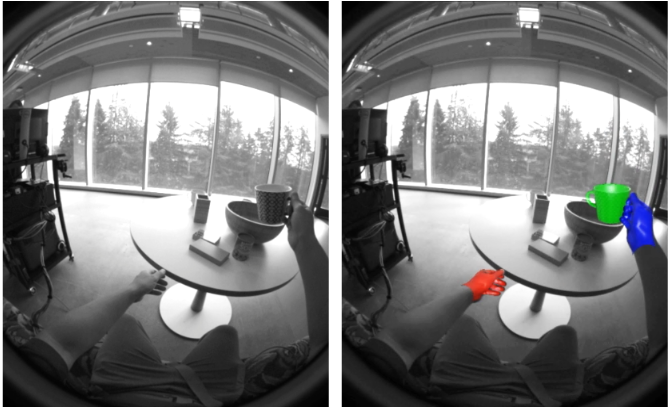
\includegraphics[width=\linewidth]{figures/SuppMat_Bad_Special.png}
    \caption{\textbf{Object annotation failure case:} Rotational ambiguity in symmetric objects.
    \textbf{Left:} The raw image from egocentric view. 
    \textbf{Right:} The projected 3D object mesh (green) overlaying the image. 
    Note that the pipeline correctly tracks the 3D position but fails to resolve the azimuthal rotation, incorrectly predicting the handle to be visible (``hallucinated'') despite not being present in the image.}
    \label{fig:failure_hallucination}
\end{figure}

\customparagraph{Impact of Action Predictability.}
The results reveal a strong correlation between the \textit{predictability} of an action and the performance gain from text conditioning. 

We observe the largest improvements in complex actions that involve specific, structured 3D state changes, such as \emph{pouring in} (38.2\% improvement), \emph{picking up} (33.9\%), and \emph{opening} (32.6\%). In these scenarios, the visual history alone may be ambiguous; for example, a hand approaching a bottle could precede lifting, opening, or sliding. The text caption serves as a strong prior that disambiguates the intent, collapsing the multimodal future distribution into a specific trajectory (e.g., the typical arc that the hand and object usually take to pour).

Conversely, actions characterized by high ambiguity or stochasticity benefit least from having text description as an additional input. In the task of predicting 6DoF object pose 30 frames ahead, \emph{inspecting} (1.1\%) and \emph{moving} (-5.2\%) show negligible or even negative differences. We attribute this to the wide variability in how users execute these actions; knowing that a user is ``inspecting'' an object predicts that the object will likely be rotated, but it does not specify the axis or magnitude of that rotation. In these high-entropy cases, the text describes the \emph{state} of the interaction but provides little kinematic signal regarding the future trajectory of the hand and object in 3D space.

This breakdown shows that the value of text-conditioning in SHOW3D is not uniform across hand-object interactions. Language features act as a high-level control signal that is most effective when the semantic intent dictates a specific kinematic protocol, effectively narrowing the search space for the forecasting model.




\section{Additional Ground Truth Examples}

We provide additional visualizations of our 3D ground truth annotations in Figure~\ref{fig:suppmat_good1}. 
These examples further illustrate the diversity of our captured environments and the high fidelity of our markerless tracking pipeline. 

\textbf{Failure Modes.} To contextualize these examples, Figure~\ref{fig:failure_cases_general} summarizes the two most common failure types observed in our automated hand annotation pipeline. The top row illustrates cases where all entities are successfully detected, but slight inaccuracies in the estimated 6DoF hand pose lead to physically implausible interpenetrations with object meshes. The bottom row shows the opposite failure mode, in which a hand is missed entirely due to heavy occlusion from the object or the opposing hand. While both issues occur infrequently relative to the dataset scale, they underscore the inherent challenges of annotating fine-grained hand–object interactions in egocentric views.

We also observe specific failure modes of our object tracking pipeline. In Figure~\ref{fig:failure_noobj}, the hands are successfully tracked but the object is missed entirely due to severe occlusion and strong outdoor illumination. In these settings, our object tracking pipeline, which relies on DINOv2~\cite{oquab2023dinov2} features, struggles when object features are either heavily occluded or when strong sunlight induces appearance changes, causing the object to go undetected by some or all cameras even when it is partially visible.

A second failure mode is shown in Figure~\ref{fig:failure_hallucination}, where the object tracking pipeline accurately localizes the 3D position of the cup but fails to estimate its azimuthal rotation, resulting in the handle being “hallucinated’’ in a visible position (right, green mesh) despite being fully occluded in the input image (left). This likely occurs because the DINOv2 features used in our pipeline~\cite{nguyen2023cnos, ornek2024foundpose, nguyen2025gotrack} are highly semantic and robust to local variations. While this robustness aids in tracking the dominant cylindrical body under occlusion, the patch-based features may lack the spatial sensitivity required to infer the orientation of the thin handle, particularly when the object appears largely rotationally symmetric.

{
    \small
    \bibliographystyle{ieeenat_fullname}
    \bibliography{main}
}

\end{document}
